\documentclass[11pt]{article}
\usepackage{mathblatt}

\makeatletter
% Überschrift (Art, Gruppe) im Kasten der nächsten Aufgabe: nie allein am Seitenende (wie \pfab)
\let\gkopf\empty
\newcommand{\gueber}[1]{\gdef\gkopf{#1}}
\newcommand{\gueberdazu}[1]{\ifx\gkopf\empty\gdef\gkopf{#1}\else\expandafter\gdef\expandafter\gkopf\expandafter{\gkopf#1}\fi}
% eingerückt (B6): \gEin Einzug, \gSchrift eine Stufe kleiner; die Überschrift bleibt ohne Einzug
\newlength{\gEin}\setlength{\gEin}{0pt}
\let\gSchrift\relax
% Ankreuzzeile mit hängendem Einzug (lange Aussagen brechen unter dem Text um, nicht unter dem Kästchen)
\renewcommand{\pfkreuzzeile}[1]{\par\noindent\hangindent3.2em\hangafter1\hspace*{1.6em}$\square$\ #1\par}
% Bauregeln 6.7: kurze Optionen in einer Zeile
\newcommand{\gkreuzreihe}[1]{\par\noindent\hspace*{1.6em}#1\par}
\newcommand{\gkreuz}[1]{$\square$\ #1\hspace{2.2em}}
% Bauregeln 6.6: links, was man ansieht, rechts, was man tut; Spaltengrenze auf dem ganzen Blatt an derselben
% Stelle (halbe Satzbreite vom linken Rand); untereinander, wenn die Skizze breiter als die linke Spalte ist
\newsavebox{\gbox}\newlength{\gLinks}
\newcommand{\gzwei}[2]{\par\smallskip\noindent\sbox{\gbox}{#1}%
  \setlength{\gLinks}{\dimexpr0.5\textwidth-\gEin-\mbpfnr\relax}%
  \ifdim\wd\gbox>\dimexpr\gLinks-4mm\relax
    \usebox{\gbox}\par\smallskip\noindent\begin{minipage}{\linewidth}#2\end{minipage}%
  \else
    \begin{minipage}[c]{\gLinks}\usebox{\gbox}\end{minipage}%
    \begin{minipage}[c]{\dimexpr\linewidth-\gLinks\relax}\raggedright #2\end{minipage}%
  \fi\par}
\RenewDocumentEnvironment{pfaufg}{m m m}{%
  \begin{lrbox}{\mbaufgabebox}\begin{minipage}[t]{\linewidth}%
  \ifx\gkopf\empty\else\noindent\gkopf\par\global\let\gkopf\empty\fi
  \gSchrift\noindent\hspace*{\gEin}\mbpfrandmarke{#1}%
  \begin{minipage}[t]{\mbpfnr}\strut\textbf{#2}\end{minipage}%
  \begin{minipage}[t]{\dimexpr\linewidth-\gEin-\mbpfnr-\mbpfbe\relax}\raggedright\strut\ignorespaces}%
 {\end{minipage}%
  \begin{minipage}[t]{\mbpfbe}\raggedleft\small\color{mbgrau}\strut#3\end{minipage}%
  \end{minipage}\end{lrbox}%
  \setlength{\mbaufgabehoehe}{\dimexpr\ht\mbaufgabebox+\dp\mbaufgabebox\relax}%
  \par\addvspace{6pt}\Needspace*{\mbaufgabehoehe}%
  \noindent\usebox{\mbaufgabebox}\par\addvspace{6pt}}
\makeatother
% Probe Serie 08.10.2026, Paket Pythagoras: Lernblatt 1 (Satz und Hypotenuse), von Hand gesetzt.
% Präambel und Makros aus bau/pruefheft/fokus-2026-10-08/dreiecke-normal-fokus-pythagoras.
% Einzelfrage geführt: grau hinterlegt, eine Frage je Schritt, darunter die Wahl mit der naheliegenden falschen Antwort
\newcommand{\efrage}[3]{\par\smallskip\noindent\colorbox{black!7}{\parbox{\dimexpr\linewidth-2\fboxsep}{\textbf{#1}\ #2\par\noindent\hspace*{1.4em}#3}}\par}
\newcommand{\kennung}{QH4}
\newcommand{\kk}[1]{$\square$\,#1\hspace{0.9em}}
\newcommand{\linie}[1]{\,{\color{black!45}\rule[-1pt]{#1}{0.4pt}}\,}

\begin{document}
\pfheftstil
\fancyfoot[C]{\parbox[t]{\textwidth}{\mbfhbox\par\vspace{1.5mm}{\footnotesize\color{mbgrau}{\scriptsize \kennung}\hfill\thepage}}}
\pfheftkopf{Die lange Seite \textperiodcentered{} Satz des Pythagoras}{Lernblatt 1}

\begin{pfaufg}{}{1.}{}
Über jeder Seite des rechtwinkligen Dreiecks steht ein Quadrat.
\gzwei{\begin{tikzpicture}[scale=0.40,line width=0.7pt,baseline=(current bounding box.north)]
\draw[mbgitter,line width=0.3pt] (-4,-3) grid (7,7);
\fill[black!10] (0,0) -- (3,0) -- (3,-3) -- (0,-3) -- cycle;
\fill[black!18] (0,0) -- (-4,0) -- (-4,4) -- (0,4) -- cycle;
\fill[black!28] (0,4) -- (3,0) -- (7,3) -- (4,7) -- cycle;
\draw (0,0) -- (3,0) -- (3,-3) -- (0,-3) -- cycle;
\draw (0,0) -- (-4,0) -- (-4,4) -- (0,4) -- cycle;
\draw (0,4) -- (3,0) -- (7,3) -- (4,7) -- cycle;
\draw[line width=1.4pt] (0,0) -- (3,0) -- (0,4) -- cycle;
\mbrwmarke{(0,0)}{(3,0)}{(0,4)}
\end{tikzpicture}}{%
\efrage{a)}{Welche Seite liegt dem rechten Winkel gegenüber?}{\gkreuz{die längste}\gkreuz{die kürzeste}}
\efrage{b)}{Wie viele Kästchen haben die zwei kleinen Quadrate?}{\gkreuz{3 und 4}\gkreuz{9 und 16}}
\efrage{c)}{Die lange Seite ist 5 Kästchen lang. Wie viele Kästchen passen in das große Quadrat?}{\gkreuz{10}\gkreuz{25}}
\efrage{d)}{Was fällt auf?}{\parbox[t]{\dimexpr\linewidth-1.4em}{$\square$\ Die zwei kurzen Seiten sind zusammen so lang wie die lange Seite.\\[1pt]$\square$\ Die zwei kleinen Quadrate haben zusammen so viele Kästchen wie das große.}}}
\fusshilfe{\mbox{1:~a) die längste; b) 9 und 16; c) 25; d) die Quadrate}}
\end{pfaufg}

\par\addvspace{4pt}
\begin{tcolorbox}[colback=white,colframe=black!45,boxrule=0.5pt,arc=1mm,left=2mm,right=2mm,top=1mm,bottom=1mm]
\small
\textbf{Hypotenuse und Katheten.} Die Seite gegenüber dem rechten Winkel heißt \textbf{Hypotenuse}; sie ist die längste Seite. Die beiden Seiten am rechten Winkel heißen \textbf{Katheten}.\par\smallskip
\textbf{Satz des Pythagoras.} Im rechtwinkligen Dreieck sind die zwei Kathetenquadrate zusammen so groß wie das Hypotenusenquadrat: \quad $a^2 + b^2 = c^2$ \quad ($c$ ist die Hypotenuse).\par\smallskip
\textbf{Hypotenuse ausrechnen:} Katheten hoch zwei, addieren, dann die Wurzel ziehen: \ $c = \sqrt{a^2 + b^2}$.\par
\hspace*{1em}$a = 5$ cm, $b = 12$ cm: \quad $c^2 = 5^2 + 12^2 = 25 + 144 = 169$ \quad $c = \sqrt{169} = 13$ cm
\end{tcolorbox}

\begin{pfaufg}{}{2.}{}
Kreuze in jedem Dreieck die Hypotenuse an.\par\smallskip\noindent
\begin{minipage}[t]{0.32\linewidth}\centering
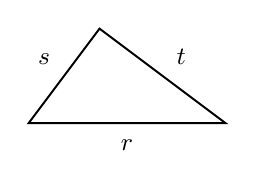
\begin{tikzpicture}[line width=0.7pt]\coordinate (P1) at (0,0);\coordinate (P2) at (2.5,0);\coordinate (P3) at (0.9,1.2);\draw (P1) -- (P2) -- (P3) -- cycle;\mbrwmarke{(P3)}{(P1)}{(P2)}
\node[font=\small,anchor=north] at (1.25,-0.08) {$r$};\node[font=\small,anchor=south east] at (0.40,0.62) {$s$};\node[font=\small,anchor=south west] at (1.75,0.62) {$t$};\end{tikzpicture}\par\smallskip
{\small a)}\ \kk{$r$}\kk{$s$}\kk{$t$}
\end{minipage}\hfill
\begin{minipage}[t]{0.32\linewidth}\centering
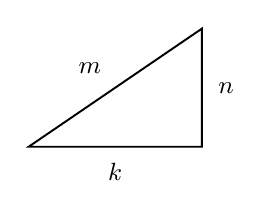
\begin{tikzpicture}[line width=0.7pt]\coordinate (P1) at (0,0);\coordinate (P2) at (2.2,0);\coordinate (P3) at (2.2,1.5);\draw (P1) -- (P2) -- (P3) -- cycle;\mbrwmarke{(P2)}{(P1)}{(P3)}
\node[font=\small,anchor=north] at (1.1,-0.08) {$k$};\node[font=\small,anchor=west] at (2.28,0.75) {$n$};\node[font=\small,anchor=south east] at (1.05,0.80) {$m$};\end{tikzpicture}\par\smallskip
{\small b)}\ \kk{$k$}\kk{$m$}\kk{$n$}
\end{minipage}\hfill
\begin{minipage}[t]{0.32\linewidth}\centering
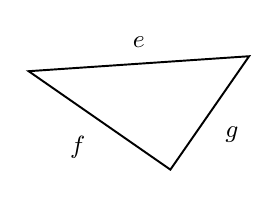
\begin{tikzpicture}[line width=0.7pt]\coordinate (P1) at (0,1.25);\coordinate (P2) at (1.8,0);\coordinate (P3) at (2.8,1.44);\draw (P1) -- (P2) -- (P3) -- cycle;\mbrwmarke{(P2)}{(P1)}{(P3)}
\node[font=\small,anchor=north east] at (0.85,0.56) {$f$};\node[font=\small,anchor=north west] at (2.37,0.67) {$g$};\node[font=\small,anchor=south] at (1.40,1.42) {$e$};\end{tikzpicture}\par\smallskip
{\small c)}\ \kk{$e$}\kk{$f$}\kk{$g$}
\end{minipage}
\fusshilfe{\mbox{2:~a) $r$; b) $m$; c) $e$}}
\end{pfaufg}

\begin{pfaufg}{P10 ’22}{3.}{}
Kreuze die Aussage an, die für jedes rechtwinklige Dreieck stimmt:
\pfkreuzzeile{Die Seite gegenüber dem rechten Winkel ist eine Kathete.}\pfkreuzzeile{$c = a + b$}\pfkreuzzeile{Die beiden Kathetenquadrate haben zusammen denselben Flächeninhalt wie das Hypotenusenquadrat.}
\fusshilfe{\mbox{3:~die dritte Aussage}}
\end{pfaufg}

\begin{pfaufg}{}{4.}{}
Schreibe den Satz des Pythagoras mit den Buchstaben des Dreiecks auf. Die Hypotenuse steht allein auf einer Seite.\par\smallskip\noindent
\begin{minipage}[t]{0.48\linewidth}
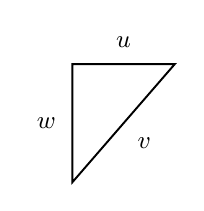
\begin{tikzpicture}[line width=0.7pt]\coordinate (P1) at (0,0);\coordinate (P2) at (0,1.5);\coordinate (P3) at (1.3,1.5);\draw (P1) -- (P2) -- (P3) -- cycle;\mbrwmarke{(P2)}{(P1)}{(P3)}
\node[font=\small,anchor=south] at (0.65,1.58) {$u$};\node[font=\small,anchor=east] at (-0.08,0.75) {$w$};\node[font=\small,anchor=north west] at (0.70,0.70) {$v$};\end{tikzpicture}\par\smallskip\noindent{\small a)}\linie{40mm}
\end{minipage}\hfill
\begin{minipage}[t]{0.48\linewidth}
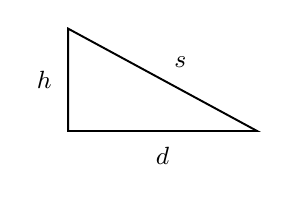
\begin{tikzpicture}[line width=0.7pt]\coordinate (P1) at (0,0);\coordinate (P2) at (2.4,0);\coordinate (P3) at (0,1.3);\draw (P1) -- (P2) -- (P3) -- cycle;\mbrwmarke{(P1)}{(P2)}{(P3)}
\node[font=\small,anchor=north] at (1.2,-0.08) {$d$};\node[font=\small,anchor=east] at (-0.08,0.65) {$h$};\node[font=\small,anchor=south west] at (1.22,0.68) {$s$};\end{tikzpicture}\par\smallskip\noindent{\small b)}\linie{40mm}
\end{minipage}
\fusshilfe{\mbox{4:~a) $u^2 + w^2 = v^2$; b) $d^2 + h^2 = s^2$}}
\end{pfaufg}

\begin{pfaufg}{nach P10 ’21}{5.}{}
Kreuze die Formel an, mit der man $z$ berechnet:
\gzwei{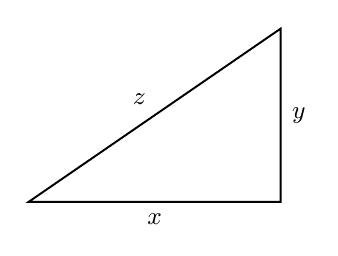
\begin{tikzpicture}[line width=0.7pt,baseline=(current bounding box.north)]\coordinate (P1) at (0.000,0.000);\coordinate (P2) at (3.200,0.000);\coordinate (P3) at (3.200,2.200);\draw (P1) -- (P2) -- (P3) -- cycle;\mbrwmarke{(P2)}{(P1)}{(P3)}\node[font=\small,anchor=west,inner sep=1.5pt] at (3.280,1.100) {$y$};\node[font=\small,anchor=south east,inner sep=1.5pt] at (1.555,1.166) {$z$};\node[font=\small,anchor=north,inner sep=1.5pt] at (1.600,-0.080) {$x$};\end{tikzpicture}}{\pfkreuzzeile{$z=\sqrt{x^2-y^2}$}\pfkreuzzeile{$z=\sqrt{x^2+y^2}$}\pfkreuzzeile{$z=\sqrt{y^2-x^2}$}\pfkreuzzeile{$z=y^2+x^2$}}
\fusshilfe{\mbox{5:~$z=\sqrt{x^2+y^2}$}}
\end{pfaufg}

\begin{pfaufg}{}{6.}{}
Ein rechtwinkliges Dreieck hat die Katheten $a = 6$ cm und $b = 8$ cm. Wie lang ist die Hypotenuse $c$?
\efrage{a)}{Was ist hier gesucht?}{\gkreuz{eine Kathete}\gkreuz{die Hypotenuse}}
\efrage{b)}{Quadriere die Katheten.}{$6^2 =$\ \gkreuz{12}\gkreuz{36}\hspace{2em}$8^2 =$\ \gkreuz{16}\gkreuz{64}}
\efrage{c)}{Wie geht es weiter?}{\gkreuz{$c^2 = 36 + 64$}\gkreuz{$c^2 = 64 - 36$}}
\efrage{d)}{Ziehe die Wurzel. Wie lang ist $c$?}{\gkreuz{100 cm}\gkreuz{50 cm}\gkreuz{10 cm}}
\fusshilfe{\mbox{6:~a) Hypotenuse; b) 36, 64; c) $c^2 = 36 + 64 = 100$; d) 10 cm}}
\end{pfaufg}

\begin{pfaufg}{}{7.}{}
Die Katheten sind $a = 36$ cm und $b = 15$ cm lang. Berechne die Hypotenuse $c$.
\par\smallskip\noindent $c^2 =$\linie{45mm}\hspace{6mm}$c =$\linie{30mm}cm
\fusshilfe{\mbox{7:~$c = 39$ cm}}
\end{pfaufg}

\begin{pfaufg}{}{8.}{}
Die Katheten sind $a = 4$ cm und $b = 9$ cm lang. Berechne die Hypotenuse $c$. Gib $c^2$ an und runde $c$ auf eine Stelle nach dem Komma.
\par\smallskip\noindent $c^2 =$\linie{45mm}\hspace{6mm}$c \approx$\linie{30mm}cm
\fusshilfe{\mbox{8:~$c \approx 9{,}8$ cm}}
\end{pfaufg}

\begin{pfaufg}{}{9.}{}
Ein Bilderrahmen ist $45$ cm breit und $24$ cm hoch. Wie lang ist seine Diagonale $d$?
\gzwei{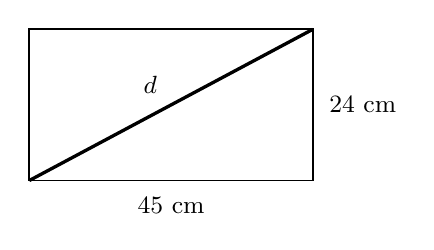
\begin{tikzpicture}[line width=0.7pt,baseline=(current bounding box.north)]\draw (0,0) rectangle (3.6,1.92);\draw[line width=1.2pt] (0,0) -- (3.6,1.92);\mbrwmarke{(3.6,0)}{(0,0)}{(3.6,1.92)}
\node[font=\small,anchor=north] at (1.8,-0.08) {$45$ cm};\node[font=\small,anchor=west] at (3.68,0.96) {$24$ cm};\node[font=\small,anchor=south east] at (1.75,0.98) {$d$};\end{tikzpicture}}{Welche Strecke ist hier die Hypotenuse?\par\gkreuz{die Seite mit 45 cm}\gkreuz{die Diagonale $d$}\rechenplatz{2}}
\fusshilfe{\mbox{9:~$d = 51$ cm}}
\end{pfaufg}

\begin{pfaufg}{nach P10 ’25}{10.}{}
Familie Yücel baut an die Stufe vor der Haustür eine Rampe für Rollstühle. Die Stufe ist $16$ cm hoch; waagerecht ist die Rampe $170$ cm lang. Berechne die Länge $x$ der Rampe.
\gzwei{\begin{tikzpicture}[line width=0.7pt,baseline=(current bounding box.north)]\coordinate (P1) at (0,0);\coordinate (P2) at (5.6,0);\coordinate (P3) at (5.6,0.62);\draw (P1) -- (P2) -- (P3) -- cycle;\mbrwmarke{(P2)}{(P1)}{(P3)}
\node[font=\small,anchor=north] at (2.8,-0.08) {$170$ cm};\node[font=\small,anchor=west] at (5.68,0.31) {$16$ cm};\node[font=\small,anchor=south] at (2.7,0.34) {$x$};
\node[font=\scriptsize,mbgrau,anchor=north west] at (0,-0.45) {nicht maßstabsgerecht};\end{tikzpicture}}{Was ist hier gesucht?\par\gkreuz{die Höhe der Stufe}\gkreuz{die schräge Rampe}\rechenplatz{2}}
\fusshilfe{\mbox{10:~$x \approx 170{,}8$ cm}}
\end{pfaufg}

\begin{pfaufg}{}{11.}{}
Lara soll die Hypotenuse $c$ berechnen. Die Katheten sind $33$ cm und $56$ cm lang. Sie rechnet so:
\gzwei{$\begin{aligned}c^2 &= 33^2 + 56^2\\ c^2 &= 4\,225\\ c &= 4\,225 \text{ cm}\end{aligned}$}{Was hat Lara falsch gemacht? Rechne richtig.\rechenplatz{2}}
\fusshilfe{\mbox{11:~Wurzel vergessen; $c = 65$ cm}}
\end{pfaufg}

\begin{pfaufg}{P10 ’20}{12.}{}
Im Dreieck $ABC$ ist bei $C$ ein rechter Winkel. Die Strecke $\overline{BC}$ ist $12$ m lang, die Strecke $\overline{AC}$ $34$ m. Berechne die Länge der Strecke $\overline{AB}$.
\gzwei{\begin{tikzpicture}[line width=0.7pt,baseline=(current bounding box.north)]\coordinate (P1) at (0.000,0.000);\coordinate (P2) at (1.200,3.400);\coordinate (P3) at (0.000,3.400);\draw (P1) -- (P2) -- (P3) -- cycle;\mbrwmarke{(P3)}{(P1)}{(P2)}\node[font=\small] at (-0.052,-0.295) {$A$};\node[font=\small] at (1.373,3.645) {$B$};\node[font=\small] at (-0.100,3.683) {$C$};\node[font=\scriptsize,mbgrau,anchor=north west] at ([yshift=-2pt]current bounding box.south west) {nicht maßstabsgerecht};\end{tikzpicture}}{\rechenplatz{4}}
\fusshilfe{\mbox{12:~$\overline{AB} \approx 36{,}1$ m}}
\end{pfaufg}

\par\vfill\noindent\begin{minipage}{\linewidth}{\scriptsize\color{mbgrau}Originale: 2020 \textperiodcentered{} 7a \quad 2021 \textperiodcentered{} 1h \quad 2022 \textperiodcentered{} 1g \quad 2025 \textperiodcentered{} 4a\par}\smallskip
{\footnotesize\color{black!70}Vorher: Quadrat und Wurzel \textperiodcentered{} Rechter Winkel im Dreieck\quad\textbullet\quad Weiter: Eine kurze Seite (Kathete)\par}\end{minipage}
\end{document}
